% --- chapter
\newcommand{\chapter}[2][]{
	\newcommand{\chapname}{#2}
	\begin{flushleft}
		\begin{minipage}[t]{\linewidth}
			
\includegraphics[height=1cm]{hdht-logo.png}
			\hspace{0pt}	
			\sffamily\bfseries\large Bài  26. Các loại quang phổ
			\begin{flushleft}
				\huge\bfseries #1
			\end{flushleft}
		\end{minipage}
	\end{flushleft}
	\vspace{1cm}
	\normalfont\normalsize
}
%-----------------------------------------------------
\chapter[Các loại quang phổ]{Các loại quang phổ}

 Mọi chất rắn, lỏng, khí được nung nóng đến nhiệt độ cao, đều phát ánh sáng. Quang phổ của ánh sáng do các chất đó phát ra gọi là quang phổ phát xạ của chúng.

\subsection{Quang phổ liên tục}

	\begin{itemize}

		\item Là một dải có màu đỏ đến tím nối liền nhau một cách liên tục.

 		\item Do các chất \textbf{rắn}, chất \textbf{lỏng} hoặc chất \textbf{khí} có áp suất lớn, phát ra khi bị nung nóng.

 		\item Quang phổ liên tục của các chất khác nhau ở cùng một nhiệt độ thì \textbf{giống nhau} và \textbf{phụ thuộc vào nhiệt độ} của chúng.
 
	\end{itemize}
\begin{center}
	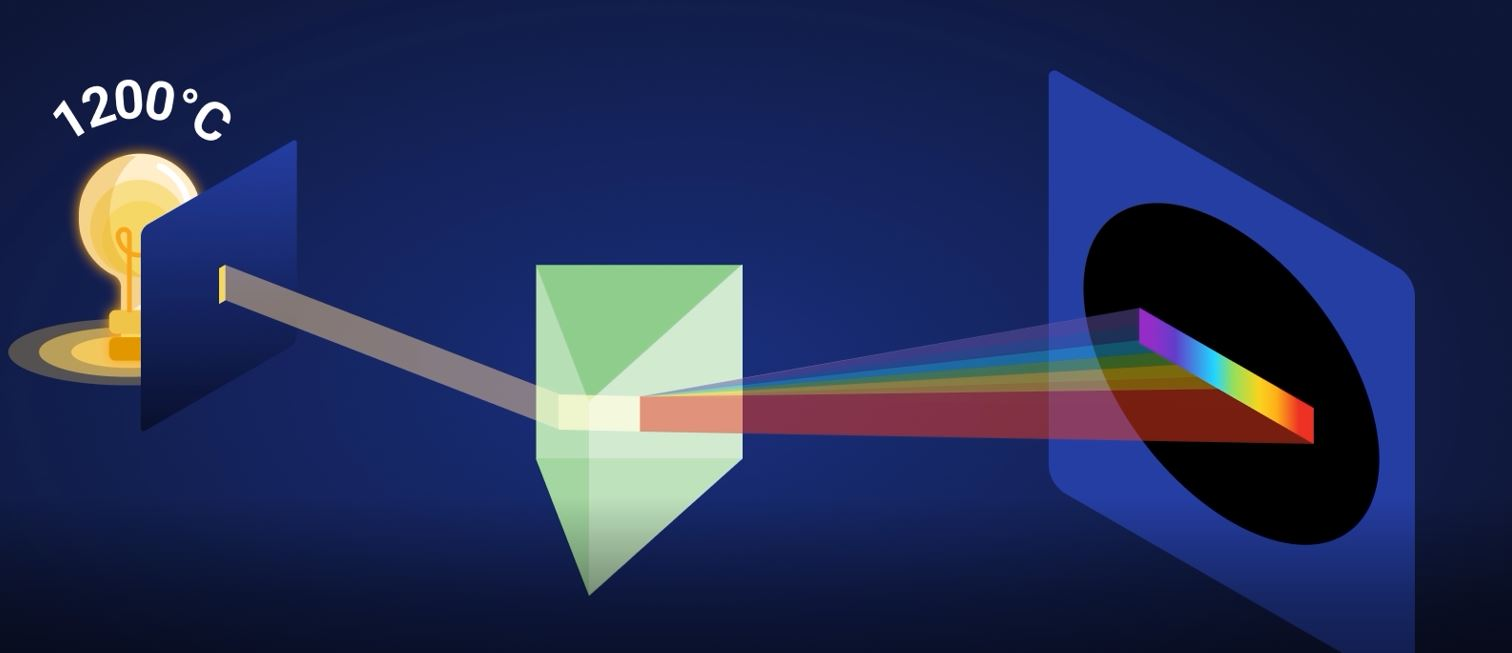
\includegraphics[width=10cm]{../figs/VN12-PH-36-L-021-2-1.JPG}
\end{center}

\subsection{Quang phổ vạch}
	
	\begin{itemize}

 		\item Là một hệ thống những \textbf{vạch sáng riêng lẻ}, ngăn cách nhau bởi những khoảng tối.

 		\item Do chất \textbf{khí ở áp suất thấp} phát ra, khi bị kích thích bằng nhiệt hay bằng điện.

 		\item Quang phổ vạch của các nguyên tố khác nhau thì \textbf{khác nhau} (số lượng các vạch, vị trí và độ sáng tỉ đối giữa các vạch).

 		\item Mỗi nguyên tố hóa học có một quang phổ vạch đặc trưng của nguyên tố đó.
 	
 	\end{itemize}
 
 \begin{center}
 	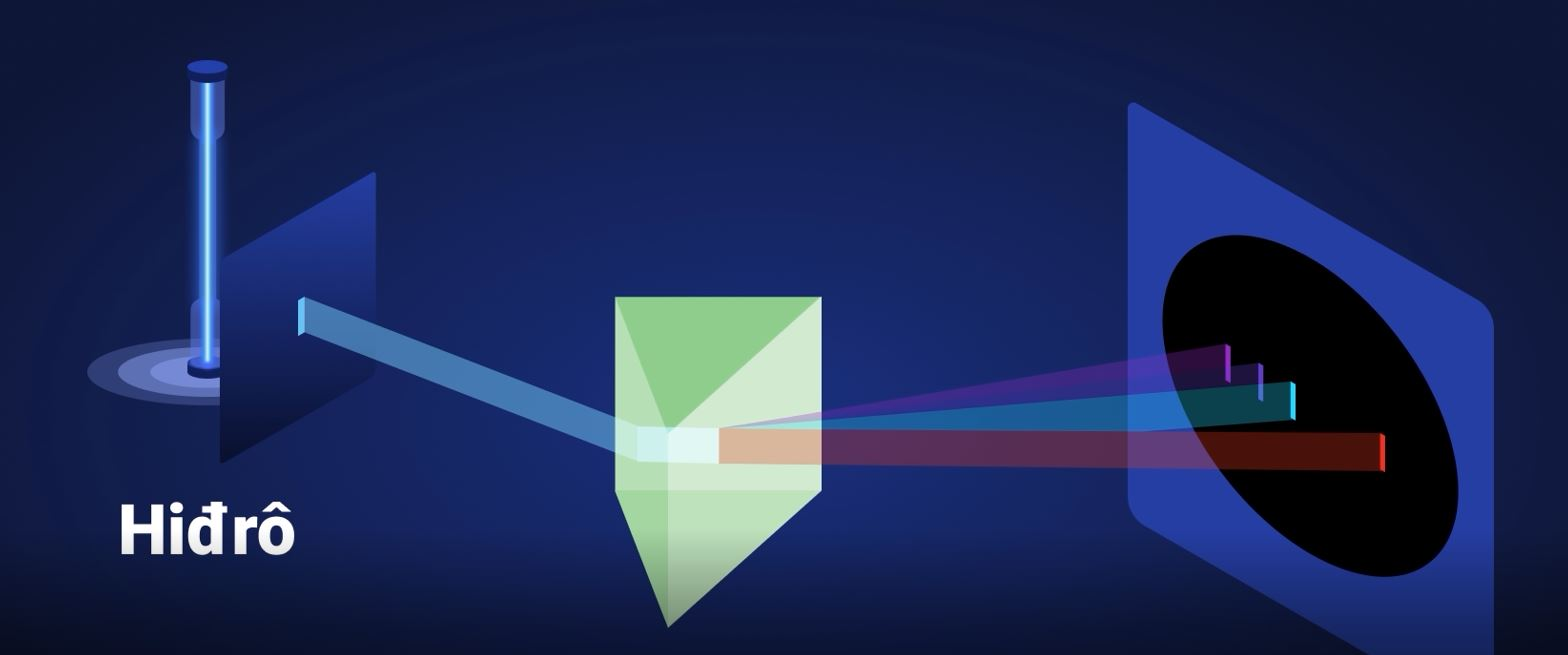
\includegraphics[width=10cm]{../figs/VN12-PH-36-L-021-2-2.JPG}
 \end{center}

	\subsubsection{Quang phổ hấp thụ}
	
	\begin{itemize}

	 	\item Là các vạch hay đám vạch tối trên nền của một quang phổ liên tục.

 		\item Điều kiện để thu được quang phổ hấp thụ là nhiệt độ của đám khí hay hơi hấp thụ phải thấp hơn nhiệt độ của nguồn sáng phát ra quang phổ liên tục.

 		\item Sự đảo sắc vạch quang phổ là sự chuyển từ một vạch sáng trên nền tối thành vạch tối trên nền sáng, do bị hấp thụ.
 	\end{itemize}
\begin{center}
	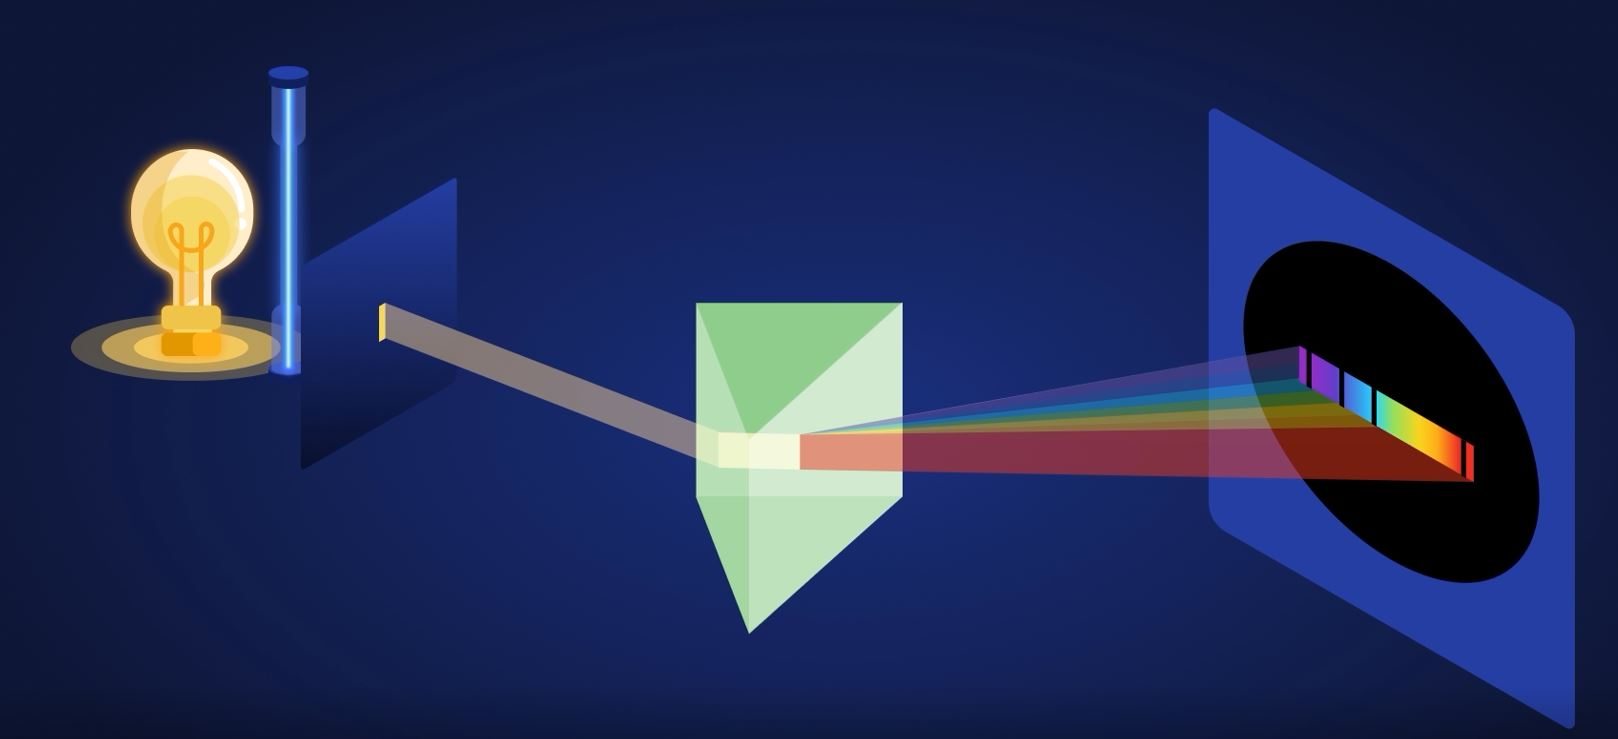
\includegraphics[width=10cm]{../figs/VN12-PH-36-L-021-2-3.JPG}
\end{center}
 \luuy{Khí hay hơi có khả năng hấp thụ các vạch ở vị trí nào thì khi phát xạ cũng phát được các vạch sáng ở vị trí đó}